%!TEX root = ../PhD_thesis__Lilian_Besson

% First chapter begins here
\chapter{Setting of This Thesis}
\label{chapter:1}
\minitoc

Abstract for Chapter 1.

\TODOL{Write this!}

\newpage
% Write miniTOC just after the title
\graphicspath{{2-Chapters/1-Chapter/Images/}}

% ----------------------------------------------------------------------------
\section{Considered problems}
\label{sec:1:problems}

\TODOL{Write this!}

\subsection{Spectrum scarcity}


\subsection{Low-consumption IoT devices for the future}


% ----------------------------------------------------------------------------
\section{Considered solutions}
\label{sec:1:solutions}

\TODOL{Write this!}


\subsection{Online/sequential machine learning to automatically improve wireless communications on the run}

\subsection{Example: Opportunistic Spectrum Access (OSA) in licensed bands}

\subsection{Example: decentralized learning in unlicensed bands with selfish or orthogonalization-based MAB algorithms}


\subsection{Reinforcement learning}

\tikzstyle{block} = [align=center, draw, fill=gray!25, rectangle, minimum height=3em, minimum width=6em]
\begin{figure}[h!]
    \centering
    \resizebox{0.40\textwidth}{!}{
        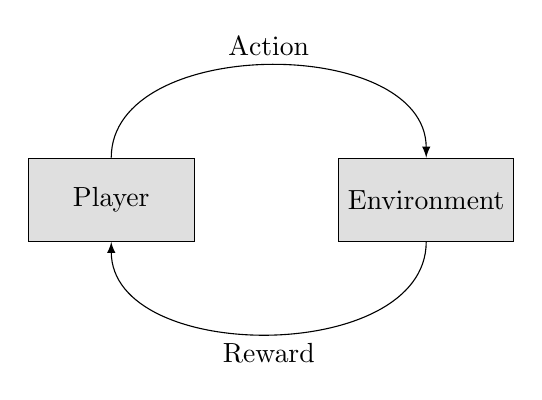
\begin{tikzpicture}[auto,node distance=5cm,>=latex,scale=2]
            %
            % We start by placing the blocks
            \node [block] (player) at (0,0) {Player};
            % We draw an edge between the player and system block to
            \node [block] (environment) at (2,0) {Environment};
            % Once the nodes are placed, connecting them is easy.
            \draw [->] (player) to[bend left=90] node[pos=0.5] {Action} (environment);
            \draw [->] (environment) to[bend left=90] node[pos=0.5] {Reward} (player);
            %
        \end{tikzpicture}
    }
\caption{Reinforcement learning cycle.}
\label{fig:1:ReinforcementLearningCycle}
\end{figure}


% ----------------------------------------------------------------------------
\section{Overview of the contributions}
\label{sec:1:contributions}

\TODOL{Write this!}

- Literature review of stochastic bandit algorithms (here)

- Aggregation of algorithms for online algorithm selection, state-of-the-art empirical performance with \textbf{Aggregator} (WCNC 2018)

- The most complete open-source simulation library for MAB problems, SMPyBandits (JMLR MLOSS and GitHub)

- Different models for MAB learning for IoT networks (CROWNCOM 2017, ICT demo 2018, WCNC 2019 and MOTIoN 2019)

- A refined analysis and a new impulse on multi-player bandits (ALT 2018, and 4-8 works inspired by our article since then). State-of-the-art with our algorithm MCTopM + klUCB for multi-player bandits "with sensing", empirical state-of-the-art with our simple (but wrong) "selfish" approach in case of "no sensing"

- Literature review on non stationary models and algorithms, state-of-the-art for piece-wise stationary with our algorithm, GLR test + klUCB

- Literature review on possible use case of doubling trick, plus a unified and more generic analysis of two families of doubling tricks !


% ----------------------------------------------------------------------------
\section{Organization of the thesis}
\label{sec:1:organization}

Here we discuss quickly the organization of the thesis.

\begin{figure}[h!]
    \centering
    \resizebox{0.85\textwidth}{!}{
    \begin{tikzpicture}[>=latex',line join=bevel,scale=3]
        %
        \node[align=center] (introduction) at (0,2.5) [rectangle,draw] {Chapter~\ref{chapter:1}\\Introduction};
        \node[align=center] (chapter2) at (0,2) [rectangle,draw] {Chapter~\ref{chapter:2}\\Multi-Armed Bandit models};
        \node[align=center] (chapter3) at (4,2) [rectangle,draw] {Chapter~\ref{chapter:3}\\SMPyBandits: simulation\\library for MAB};
        \node[align=center] (chapter4) at (-2,1) [rectangle,draw] {Chapter~\ref{chapter:4}\\Two MAB models for IoT networks};
        \node[align=center] (chapter5) at (0,1) [rectangle,draw] {Chapter~\ref{chapter:5}\\Multi-players MAB};
        \node[align=center] (chapter6) at (2,1) [rectangle,draw] {Chapter~\ref{chapter:6}\\Non-stationary MAB models};
        \node[align=center] (conclusion) at (0,0) [rectangle,draw] {Chapter~\ref{chapter:conclusion}\\General conclusion};
        %
        \draw [color=black,thick,->] (introduction) to (chapter2);
        \draw [color=black,thick,<->] (chapter2) to (chapter3);
        \draw [color=black,thick,->] (chapter2) to (chapter4);
        \draw [color=black,thick,->] (chapter2) to (chapter5);
        \draw [color=black,thick,->] (chapter2) to (chapter6);
        \draw [color=black,thick,->] (chapter4) to (conclusion);
        \draw [color=black,thick,->] (chapter5) to (conclusion);
        \draw [color=black,thick,->] (chapter6) to (conclusion);
        %
    \end{tikzpicture}
    }
    \caption{Organization of the thesis.}
    \label{fig:1:organization}
\end{figure}


% ----------------------------------------------------------------------------
\section{List of publications}
\label{sec:1:listPublications}

% =============================================================================
\subsection{Publications in international conferences with proceedings}

\begin{itemize}
\item
    \emph{GNU Radio Implementation of MALIN: ``Multi-Armed bandits Learning for Internet-of-things Networks''},
    by \textbf{Lilian Besson}, Rémi Bonnefoi \& Christophe Moy.
    \emph{Wireless Communication and Networks Conference} (IEEE WCNC, \href{http://wcnc2019.ieee-wcnc.org}{\texttt{wcnc2019.ieee-wcnc.org}}), Marrakech, Morocco, April 2019,
    \href{https://HAL.Inria.fr/hal-02006825}{\texttt{HAL.Inria.fr/hal-02006825}}.
    \cite{Besson2019WCNC}

\item
    \emph{Multi-Player Bandits Revisited},
    by \textbf{Lilian Besson} \& Emilie Kaufmann.
    \emph{Algorithmic Learning Theory} (ALT, \href{http://www.cs.cornell.edu/conferences/alt2018}{\texttt{www.cs.cornell.edu/conferences/alt2018}}), Lanzarote, Spain, April 2018,
    \href{https://HAL.Inria.fr/hal-01629733}{\texttt{HAL.Inria.fr/hal-01629733}}.
    \cite{Besson2018ALT}

\item
    \emph{Aggregation of Multi-Armed Bandits learning algorithms for Opportunistic Spectrum Access},\\
    by \textbf{Lilian Besson}, Emilie Kaufmann \& Christophe Moy.
    \emph{Wireless Communication and Networks Conference} (IEEE WCNC, \href{http://wcnc2018.ieee-wcnc.org}{\texttt{wcnc2018.ieee-wcnc.org}}), Barcelone, Spain, April 2018,
    \href{https://HAL.Inria.fr/hal-01705292}{\texttt{HAL.Inria.fr/hal-01705292}}.
    \cite{Besson2018WCNC}

\item
    \emph{Multi-Armed Bandit Learning in IoT Networks and non-stationary settings},
    by Rémi Bonnefoi, \textbf{Lilian Besson}, Christophe Moy, Emilie Kaufmann \& J. Palicot.
    \emph{Conference on Cognitive Radio Oriented Wireless Networks} (CROWNCOM, \href{http://crowncom.org/2017}{\texttt{crowncom.org/2017}}), Lisboa, Portugal, Septembre $2017$,
    \href{https://HAL.Inria.fr/hal-01575419}{\texttt{HAL.Inria.fr/hal-01575419}},
    \textbf{Best Paper Award}.
    \cite{Bonnefoi17}

\end{itemize}

% =============================================================================
\subsection{Publications in international conferences without proceedings}

\begin{itemize}

\item
    \emph{Decentralized Spectrum Learning for IoT Wireless Networks Collision Mitigation},\\
    by Christophe Moy \& \textbf{Lilian Besson}.
    1st International ISIoT workshop (\href{https://sites.google.com/view/ISIoT2019}{\texttt{sites.google.com/view/ISIoT2019}}),
    at \emph{Conference on Distributed Computing in Sensor Systems} (IEEE DCOSS, \href{http://2019.dcoss.org}{\texttt{2019.dcoss.org}}), Santorini, Greece, May 2019.
    \cite{MoyBesson2019}

\item
    \emph{Upper-Confidence Bound for Channel Selection in LPWA Networks with Retransmissions},\\
    by Rémi Bonnefoi, \textbf{Lilian Besson}, J. Manco-Vasquez \& Christophe Moy.
    1st International MOTIoN workshop (\href{https://sites.google.com/view/wcncworkshop-motion2019}{\texttt{sites.google.com/view/wcncworkshop-motion2019}}),
    at \emph{Wireless Communication and Networks Conference} (IEEE WCNC, \href{http://wcnc2019.ieee-wcnc.org}{\texttt{wcnc2019.ieee-wcnc.org}}), Marrakech, Morocco, April 2019.
    \cite{Bonnefoi2019WCNC}

\item
    \emph{MALIN: ``Multi-Arm bandit Learning for Iot Networks'' with GRC: A TestBed Implementation and Demonstration that Learning Helps},
    by \textbf{Lilian Besson}, Rémi Bonnefoi, Christophe Moy.
    Demonstration presented at \emph{International Conference on Communication} (ICT, \href{http://ict-2018.org/demos}{\texttt{ict-2018.org/demos}}), in Saint-Malo, France in June $2018$.
    See \href{https://YouTu.be/HospLNQhcMk}{\texttt{YouTu.be/HospLNQhcMk}} for a $6$-minutes presentation video.
    \cite{Besson2018ICT}

\end{itemize}


% =============================================================================
\subsection{Submitted works}

\begin{itemize}
\item
    \emph{Analyse non asymptotique d'un test séquentiel de détection de ruptures et application aux bandits non stationnaires} (in French),
    submitted at GRETSI 2019, \href{http://GRETSI.fr/colloque2019}{\texttt{GRETSI.fr/colloque2019}},
    by \textbf{Lilian Besson} \& Emilie Kaufmann, March $2019$,
    \href{https://HAL.Inria.fr/hal-02006471}{\texttt{HAL.Inria.fr/hal-02006471}}.
    \cite{Besson2019Gretsi}

\end{itemize}


% =============================================================================
\subsection{In progress works waiting for a new submission}

\begin{itemize}

\item
    \emph{The Generalized Likelihood Ratio Test meets klUCB: an Improved Algorithm for Piece-Wise Non-Stationary Bandits},
    by \textbf{Lilian Besson} \& Emilie Kaufmann, February $2019$,
    \href{https://HAL.Inria.fr/hal-02006471}{\texttt{HAL.Inria.fr/hal-02006471}}.
    \cite{Besson2019GLRT}

\item
    \emph{SMPyBandits: an Open-Source Research Framework for Single and Multi-Players Multi-Arms Bandits (MAB) Algorithms in Python},
    by \textbf{Lilian Besson}, active development since October $2016$,
    \href{https://HAL.Inria.fr/hal-01840022}{\texttt{HAL.Inria.fr/hal-01840022}}.
    About $40000$ lines of code, hosted on \href{https://GitHub.com/SMPyBandits}{\texttt{GitHub.com/SMPyBandits}},
    with a complete documentation on \href{https://SMPyBandits.rtfd.io}{\texttt{SMPyBandits.rtfd.io}}.
    \cite{SMPyBandits,SMPyBanditsJMLR}

\item
    \emph{What Doubling-Trick Can and Can't Do for Multi-Armed Bandits},\\
    by \textbf{Lilian Besson} \& Emilie Kaufmann, September $2018$,
    \href{https://HAL.Inria.fr/hal-01736357}{\texttt{HAL.Inria.fr/hal-01736357}}.
    \cite{Besson2018DoublingTricks}

\end{itemize}


% =============================================================================
\subsection{Other works}

\begin{itemize}
\item
    \emph{A Note on the Ei Function and a Useful Sum-Inequality},
    by \textbf{Lilian Besson},
    February $2018$,
    \href{https://HAL.Inria.fr/hal-01847480}{\texttt{HAL.Inria.fr/hal-01847480}}.

\end{itemize}


% =============================================================================
\subsection{Presentations in seminars and conferences}

\paragraph{Seminars}
    I gave some presentations in the following events:
    SequeL team seminar at Inria Lille in September and December $2017$, and June $2019$;
    SCEE team seminar at CentraleSupélec, Rennes campus, in October $2017$, February $2018$ and June $2019$;
    as well as
    for the GDR ISIS day held in Issy-les-Moulineaux on November $2017$,
    for the brown-bag seminar at ENSAI in Bruz in January $2018$,
    for the weekly seminar at CMAP lab at École Polytechnique in October $2018$,
    for the weekly seminar of the PANAMA project-team at IRISA / Inria Rennes in May $2019$.

\paragraph{Tutorial}
    I gave a tutorial\footnote{Cf. \href{HAL.Inria.fr/cel-01830248}{\texttt{HAL.Inria.fr/cel-01830248}}} on the Julia language, at IETR seminar in Vannes in June $2018$,
    with Pierre Haessig (\texttt{pierreh.eu}).

\paragraph{Training}
    I was also in charge of ``GouTP'' training sessions for about $30$ PhD students at CentraleSupélec Rennes.
    We had a lot of various $1$h training sessions between January $2017$ and June $2019$,
    and I gave about $12$ training sessions, on various topics including Python, \texttt{git}, HAL and arXiv, the Julia language and Bib\TeX{}.


% =============================================================================
\subsection{Other experiences}

\paragraph{Conferences}
    I attended the following conferences:
	\emph{International Conference on Communication} ICC (Paris), May $2017$,
    \emph{Conference on Learning Theory} COLT (Amsterdam), July $2017$,
    \emph{Conference on Cognitive Radio Oriented Wireless Networks} CROWNCOM (Lisboa), September $2017$,
    \emph{Conference on Algorithmic Learning Theory} ALT (Lanzarote), April $2018$,
    \emph{Wireless Communication and Networking Conference} WCNC (Barcelona), April $2018$,
	\emph{International Conference on Telecommunication} ICT (Saint-Malo), June $2018$,
    \emph{Wireless Communication and Networking Conference} WCNC (Marrakech), April $2019$,
    \emph{Colloque francophone de traitement du signal et des images} GRETSI (Lille), August $2019$.

\paragraph{Seminars}
    I attended the following seminars:
	\emph{Workshop Learn with Earning} (Rotterdam), May $2018$,
	\emph{Workshop on Optimization and Learning} (Toulouse), September $2018$,
	\emph{European Workshop on Reinforcement Learning} (Lille), October $2018$,

\paragraph{Responsabilities}
    I was the president of the PhD Students Association of IETR lab (ADDI, \texttt{addi.asso.insa-rennes.fr}) in $2017$.
    I was notably in charge of organizing the PhD Students day at Rennes, in June $2017$, with about $350$ people, and presentation of a research poster\footnote{Cf. \href{https://HAL.Inria.fr/hal-02013839}{\texttt{HAL.Inria.fr/hal-02013839}}}
    I also helped for the organization and presented another poster\footnote{Cf. \href{https://HAL.Inria.fr/hal-02013847}{\texttt{HAL.Inria.fr/hal-02013847}}} at the ``IETR : Interagir Evaluer Transmettre Réunir'' seminar, held in Vannes in June $2018$.

\paragraph{Reviews}
	for \emph{European Workshop on Reinforcement Learning} (Lille) \href{https://ewrl.wordpress.com/ewrl14-2018}{\texttt{ewrl.wordpress.com/ewrl14-2018}}, in October $2018$, I reviewed $5$ papers.
	I helped colleagues for articles submitted at international conferences \emph{AISTATS} $2019$, \emph{NeurIPS} $2017$ et $2018$, and \emph{COLT} $2018$ and $2019$, for about 10 \emph{reviews}.

\paragraph{System Administrator}
	maintaining our workstations running GNU/Linux and Windows
	at SCEE team,
	and our cognitive radio test-bed using USRP cards and the GNU Radio software,
	from January $2017$ to September $2018$.

